\documentclass{minimal}

% Tikz
\usepackage{pgf}
\usepackage{tikz}

\begin{document}

\begin{center}
 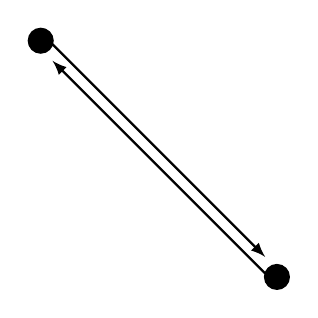
\begin{tikzpicture}
 [
 	vertex/.style={draw=none,circle,fill=black,minimum size=2pt},
	oedge/.style={->,>=latex,shorten >=6pt,draw,black,thick},
	roedge/.style={->,>=latex,shorten >=6pt,draw,black,thick,color=red}
 ]

\coordinate (V1) at (-3,3);
\coordinate (V2) at (0,0);

\path[oedge] ([yshift=3pt]V1) to ([yshift=3pt]V2) {};
\path[oedge] ([yshift=-3pt]V2) to ([yshift=-3pt]V1) {};

\node[vertex] at (V1) {};
\node[vertex] at (V2) {};

\end{tikzpicture}
\end{center}

\end{document}
